\documentclass[UTF8,ctexart,a4paper,11pt,openany]{article}
\usepackage[slantfont,boldfont]{xeCJK}
\usepackage{fontspec}
\usepackage{ctex}

\setCJKmainfont{SimSun}%[BoldFont=SimHei] %去掉注释:bf 字体为黑体

\setsansfont{SimHei}
\setCJKsansfont{SimHei}

\xeCJKsetcharclass{"2160}{"2470}{1}% 1: CJK
\xeCJKsetup{AutoFallBack=true}
\setCJKfallbackfamilyfont{\CJKrmdefault}{SimSun.ttf}

%\setmainfont{Times New Roman}     %去掉注释:Times new roman 字体
%\usepackage{mathptmx}             %去掉注释:Times new roman 字体
\usepackage{longtable}
\usepackage{mathtools}
\usepackage{amsmath}
\usepackage{amsfonts}
\usepackage{amssymb}
\usepackage{amsthm}
\usepackage[T1]{fontenc}
\usepackage{indentfirst} %段首空两格


\usepackage{graphicx}
\usepackage{geometry}
\usepackage{latexsym}
\usepackage{fancyhdr}
\usepackage{epstopdf}
%\usepackage{pifont}
%\usepackage[perpage,symbol*]{footmisc}
\usepackage{titlesec}
\usepackage{setspace}
\usepackage{enumerate}
\usepackage{enumitem}
\usepackage{multicol}
\usepackage{url}
\usepackage{exscale}
\usepackage{ulem}
\usepackage{relsize}
\usepackage{mathrsfs}
\usepackage{tikz}
\usepackage{wrapfig}
\usepackage{framed}
\usepackage{bm}
%\usepackage{pstricks,pst-node,multido,ifthen,calc}
\usepackage[all]{xy}
\usepackage{extarrows}
%\usepackage[backref]{hyperref}
\usepackage{hyperref}
\usepackage{stfloats} %插图的时候不分页

\setlength{\parindent}{2em} %段首空两格
\linespread{1.2}
\usepackage{listings}
\usepackage{xcolor}
\usepackage{algorithm}
\usepackage{algorithmicx}
\usepackage{algpseudocode}
\usepackage{mdframed}
\usepackage{extarrows}
\usepackage{diagbox}
\usepackage{makecell}
\usepackage{pgfplots}
\usepackage{csvsimple}
\theoremstyle{definition}
\mdfdefinestyle{theoremstyle}{%
linecolor=orange!40,linewidth=.5pt,%
backgroundcolor=orange!10,
skipabove=8pt,
skipbelow=5pt,
innerleftmargin=7pt,
innerrightmargin=7pt,
frametitlerule=true,%
frametitlerulewidth=.5pt,
frametitlebackgroundcolor=orange!35,
frametitleaboveskip=0pt,
frametitlebelowskip=0pt,
innertopmargin=.4\baselineskip,
innerbottommargin=.4\baselineskip,
shadow=true,shadowsize=3pt,shadowcolor=black!20,
%theoremseparator={\hspace{1pt}},
theoremseparator={.},
nobreak=true,
}


\everymath{\displaystyle}

\newtheorem{definition}{\hspace{2em}定义}[section]
\newtheorem{axiom}{\hspace{2em}公理}

\mdtheorem[style=theoremstyle]{theorem}{定理}
\mdtheorem[style=theoremstyle]{example}{例}
\mdtheorem[style=theoremstyle]{exercise}{问题}
\newtheorem{lemma}[theorem]{\hspace{2em}引理}
\newtheorem{corollary}[theorem]{\hspace{2em}推论}

\newcommand*{\QED}{\hfill\ensuremath{\square}}
\newcommand*{\rmk}{\textbf{注:}}
\renewcommand*{\proof}{\textbf{证明:}}
\newcommand*{\tips}{\textbf{提示:}}
\newcommand*{\hard}{\textbf{\color{red}(难)}}
\newcommand*{\eqsmall}{\setlength\abovedisplayskip{1pt}\setlength\belowdisplayskip{1pt}}
\geometry{left=2cm,right=2cm,top=2cm,bottom=2cm}
\title{数理统计大作业}
\author{GoodMorning29}
\pagestyle{fancy}
\fancyfoot[C]{}
\fancyhead[RO]{ \thepage}
\fancyhead[LE]{\thepage  }

\titleformat{\chapter}{\centering\huge\bfseries}{第\,\thechapter\,章}{1em}{} %更改标题样式
\titleformat{\section}{\bfseries\Large}{$\S$\,\thesection\,}{1em}{} %更改标题样式
\titlespacing*{\chapter}{0pt}{9pt}{0pt} %调整标题间距
\setenumerate[1]{itemsep=0pt,partopsep=0pt,parsep=\parskip,topsep=0pt} %设置 enumerate 行间距
\setenumerate[2]{itemsep=0pt,partopsep=0pt,parsep=\parskip,topsep=0pt} %设置 enumerate 行间距
\setitemize[1]{itemsep=0pt,partopsep=0pt,parsep=\parskip,topsep=0pt} % 设置 itemize 行间距
\setlist[enumerate,2]{label=(\arabic*),topsep=0mm,itemsep=0mm,partopsep=0mm,parsep=\parskip}
    % 设置二层枚举为 (1) 样式
    
\newfontfamily\hei{SimHei}
\newcommand\textcf[1]{\textbf{\textsf{\hei{#1}}}}

\newcommand\e{\leftarrow}
%\renewcommand{\bibname}{参考文献}

\begin{document}

\begin{center}
{\huge \textbf{数理统计大作业}}

{\large GoodMorning29}

修订日期:2024 年 12 月 25 日
\end{center}

\section{问题描述}
在本次报告中,我们将研究影响 covid-19 的因素数据,数据来源自
\url{https://cmu-delphi.github.io/delphi-epidata/api/covidcast-signals/fb-survey.html}
变量包含 COVID-19 病例指数,流感样症状,家庭社区病例指数的加权平均值,口罩有效性信念加权平均值,社交距离有效性信念加权平均值,已接种 COVID 疫苗朋友数量加权平均值,室内大型活动可能性加权平均值,公共场所他人戴口罩加权平均值,公共场所他人保持社交距离加权平均值,室内购物可能性加权平均值,室内用餐可能性加权平均值,担心感染 COVID-19 加权平均值,家庭社区病例指数平均值,没有家庭社区病例指数数量,过去 7 天中戴口罩人数,使用公共交通人数,担心财务状况人数,测试结果阳性人数

\section{描述性统计分析}
通过使用 describe 函数,我们可以得到数据的描述性统计信息,如下表所示:
\begin{table}[H]
\centering
\small
\csvautotabular{../stats_summary.csv}
\end{table}
以测试结果阳性人数为例,可以发现其大致遵循正态分布。
\begin{figure}[H]
\centering
\begin{minipage}{0.45\textwidth}
    \centering
    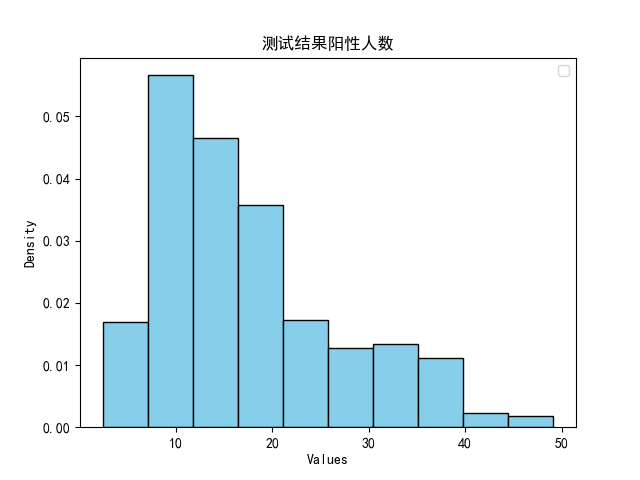
\includegraphics[width=\textwidth]{Figure_1.png}
    \caption{测试结果阳性人数分布图}
    \label{fig:positive_cases}
\end{minipage}
\hfill
\begin{minipage}{0.45\textwidth}
    \centering
    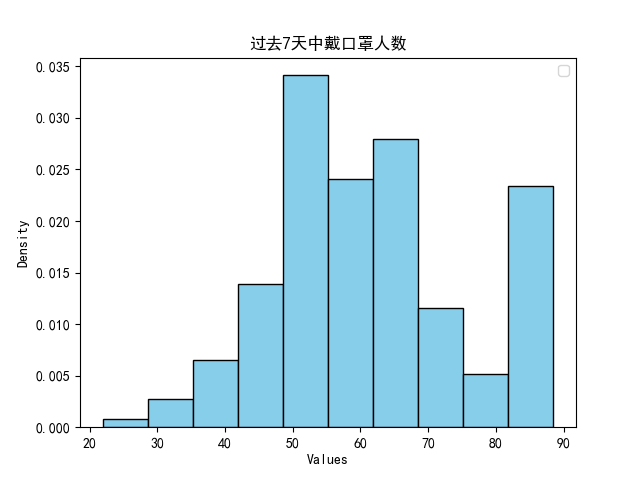
\includegraphics[width=\textwidth]{Figure_2.png}
    \caption{七天内戴口罩人数分布图}
    \label{fig:mask_wearing}
\end{minipage}
\end{figure}
再查看七天内戴口罩的人数,其分布并没有“中间多,两边少”的特点,
这可能是因为过去七天中发生了一些特殊事件,导致人们的行为发生了变化。
\section{统计推断}
\subsection{分布函数的估计}
由于因素过多,我们此处以担心感染 covid19 加权平均值数据为例,
绘制数据的核密度估计(Kernel Density Estimation, KDE)曲线,以及
正态分布拟合曲线,如下图所示:
\begin{figure}[H]
\centering
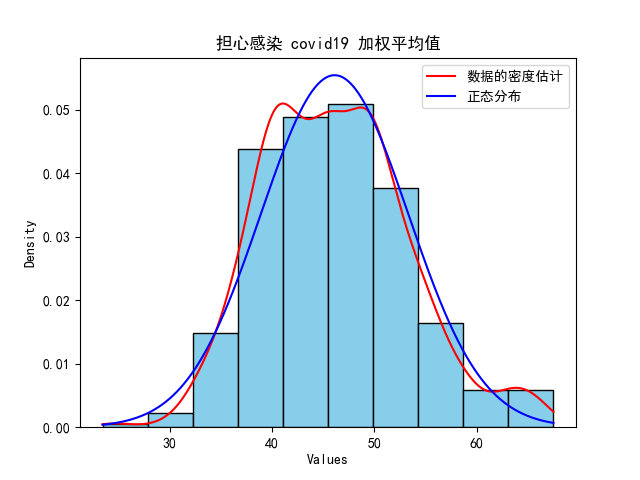
\includegraphics[width=0.6\textwidth]{Figure_3.png}
\caption{担心感染 covid19 加权平均值数据的核密度估计曲线}
\label{fig:kde}
\end{figure}
可以看出,其分布与正态分布较接近,我们可以求出置信度为
95\% 的置信区间,如下所示:
\begin{align*}
\text{均值的置信区间} & : \left( \bar{\xi} - t_{\alpha/2} \frac{S}{\sqrt{n}}, \bar{\xi} + t_{\alpha/2} \frac{S}{\sqrt{n}} \right) \\
\text{方差的置信区间} & : \left( \frac{(n-1)s^2}{\chi^2_{1-\alpha/2}(n-1)}, \frac{(n-1)s^2}{\chi^2_{\alpha/2}(n-1)} \right)
\end{align*}
得到均值置信水平为 0.95 的置信区间为:(45.79362500004988, 46.42556521629917),
置信水平为 0.95 的方差置信区间为:(48.69075245509998, 55.130121666086886)
\subsection{检验}
在 Python 中,我们可以用 probplot 函数绘制 Q-Q 图,以检验数据是否符合正态分布。
\begin{figure}[H]
\centering
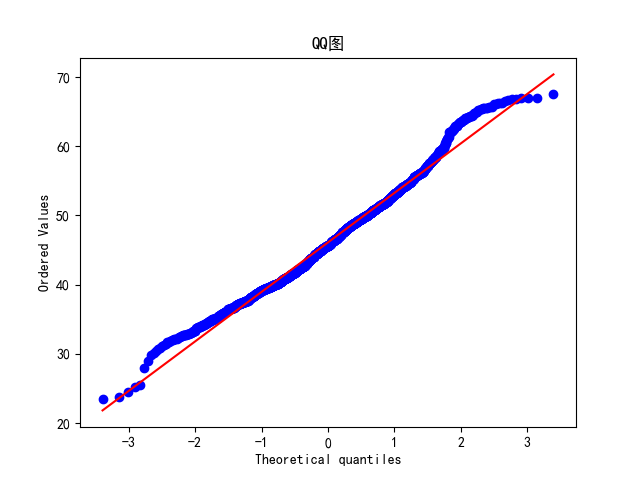
\includegraphics[width=0.6\textwidth]{Figure_4.png}
\caption{Q-Q 图}
\label{fig:qq}
\end{figure}
从图中可以看出,除两端数据点有偏差以外,数据点基本在直线上。同时我们可以绘制出
其经验曲线和正态分布曲线,可以发现其大体符合正态分布。
\begin{figure}[H]
\centering
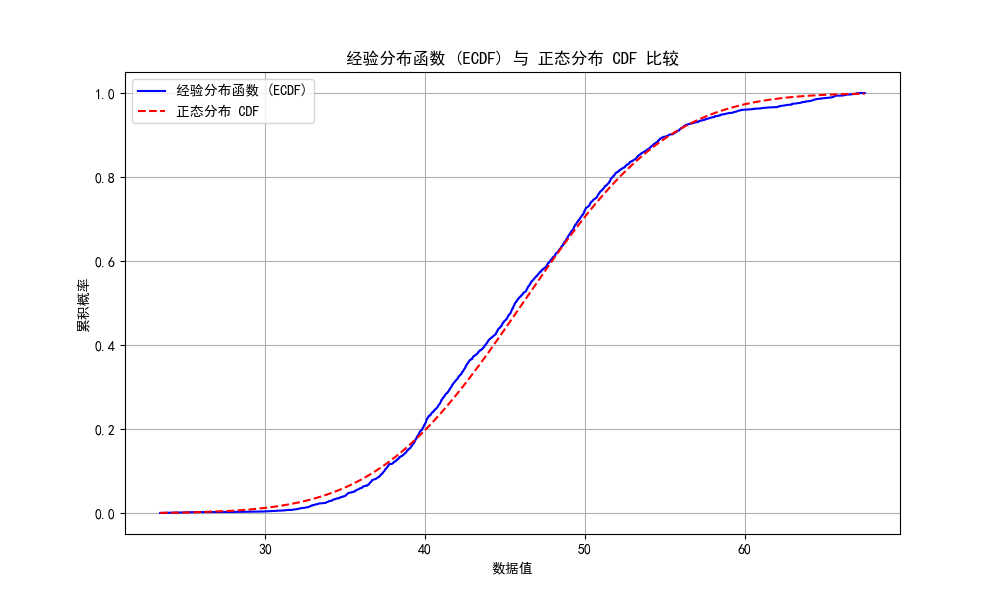
\includegraphics[width=0.8\textwidth]{Figure_5.png}
\caption{经验曲线和正态分布曲线}
\label{fig:ecdf}
\end{figure}
但是通过 kurtosis 和 normaltest 函数进行峰度值和偏度值的检验,我们发现数据并不符合正态分布。\par   
数据的偏度值:0.3728307323760319\par
数据的峰度值:0.1013558431733732\par
偏度显著性检验的统计量:44.586417382085095, p 值:2.080570716267187e-10\par
故正态性分析结果为:
拒绝原假设,数据显著偏离正态分布。
数据右偏(正偏)。
数据具有较低的峰度,分布较平坦。
\section{方差分析}

以七天内佩戴口罩为例,我们想知道佩戴口罩对检测为阳性的人数是否有影响。
按照等距分组,我们将数据依据佩戴口罩人数分为 4 组,进行方差分析。
通过调用函数 anova\_lm 可以得到方差分析表,如下所示:
\[
\begin{array}{|c|c|c|c|c|c|}
\hline
\textbf{方差来源} & \textbf{平方和} & \textbf{自由度} & \textbf{样本方差} & \textbf{F 值} & \textbf{p 值} \\
\hline
\text{因素 (Factor: C(mask\_group))} & 12475.625198 & 3 & 4158.541733 & 50.130206 & 3.133201 \times 10^{-31} \\
\hline
\text{误差 (Error)} & 165080.071944 & 1990 & 82.954810 & - & - \\
\hline
\text{总和 (Total)} & 177555.697142 & 1993 & - & - & - \\
\hline
\end{array}
\]
可以看出,F=50.130206>$F_{0.05}(3,1990)\approx 0.12$,p 值为 $3.133201 \times 10^{-31}$,拒绝原假设,即佩戴口罩人数对检测为阳性的人数有显著影响。
\section{回归分析}
\subsection{相关性及其度量}\par
在进行相关分析和回归分析之前,可先通过不同变量之间的散点图直观地了解它们之间的关系和相关程度。若图中数据点分布在一条直线(曲线)附近,表明可用直线(曲线)近似地描述变量间的关系。若有多个变量,常制作多幅两两变量间的散点图来考察变量间的关系。
先以家庭社区病例指数平均值和为例,画出散点图。Pyhon 中使用函数 plot( ) 可以方便地画出两个样本的散点图,从而直观地了解对应随机变量之间的相关关系和相关程度。输出结果如下
\begin{figure}[H]
\centering
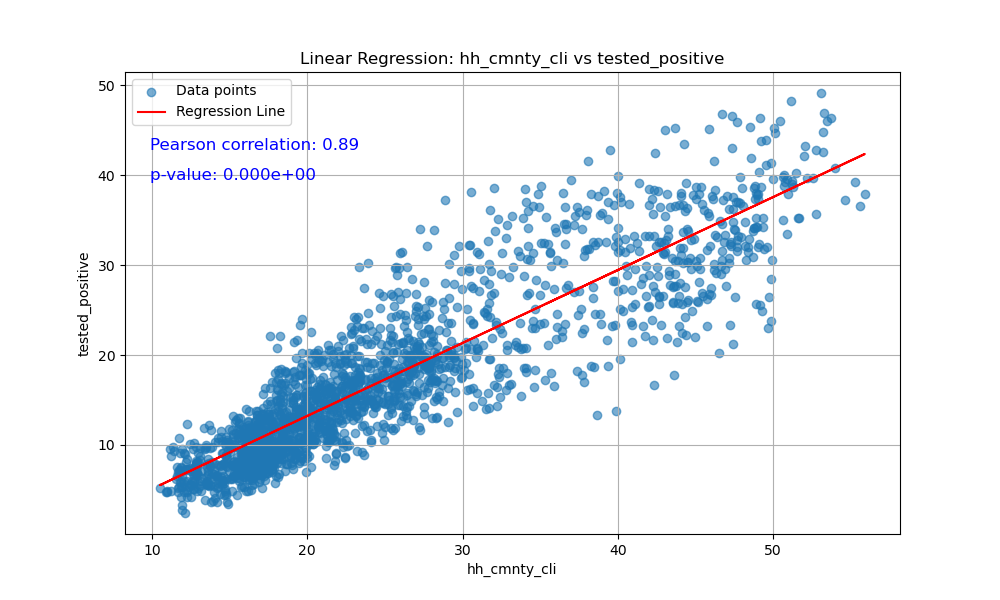
\includegraphics[width=0.8\textwidth]{Figure_6.png}
\caption{家庭社区病例指数平均值与测试结果阳性人数的散点图}
\label{fig:scatter}
\end{figure}
从图中可以看出,家庭社区病例指数平均值与测试结果阳性人数之间存在一定的线性关系。\par
进一步,它们之间的相关性可以用 Pearson 相关系数来度量。Pearson 相关系数是用来度量两个变量之间的线性相关程度的统计量,其值介于 -1 和 1 之间。当相关系数为 1 时,表示两个变量之间存在完全的正线性关系;当相关系数为 -1 时,表示两个变量之间存在完全的负线性关系;当相关系数为 0 时,表示两个变量之间不存在线性关系。在 Python 中,可以使用函数 corrcoef( ) 来计算两个变量之间的相关系数。输出结果如下:
\begin{align*}
    \text{Pearson correlation coefficient} & : 0.89 \\
    \text{p-value} & : 0.000
\end{align*}
由于 p-value 小于 0.05,故可以认为家庭社区病例指数平均值与测试结果阳性人数之间存在显著的线性相关关系。\par
\subsection{一元线性回归分析}
可以通过调用 statsmodels 包中的 OLS 函数来进行一元线性回归分析。可以通过调用函数 summary( ) 来查看回归分析的结果。输出结果如下:
\begin{longtable}{|c|c|c|c|c|}
    \hline
    \textbf{系数 (Coef.)} & \textbf{标准误差 (Std. Err.)} & \textbf{t 值 (t)} & \textbf{p 值 (P>|t|)} & \textbf{95\% 置信区间 (95\% Conf. Interval)} \\
    \hline
    \endfirsthead
    \hline
    \textbf{系数 (Coef.)} & \textbf{标准误差 (Std. Err.)} & \textbf{t 值 (t)} & \textbf{p 值 (P>|t|)} & \textbf{95\% 置信区间 (95\% Conf. Interval)} \\
    \hline
    \endhead
    \hline
    \text{常数项 (const)} & -2.9848 & 0.248 & -12.019 & [ -3.472, -2.498 ] \\
    \hline
    \text{hh\_cmnty\_cli} & 0.8107 & 0.009 & 89.000 & [ 0.793, 0.829 ] \\
    \hline
    \end{longtable}
    
    \textbf{回归模型摘要:}\par
    \begin{tabular}{|llll|}
        \hline
        \textbf{依赖变量} & 测试阳性 (tested\_positive) & \textbf{Omnibus 检验值} & 120.957 \\
        \textbf{R 平方} & 0.799 & \textbf{Omnibus 的 p 值} & 0.000 \\
        \textbf{调整后的 R 平方} & 0.799 & \textbf{Jarque-Bera 检验值} & 211.775 \\
        \textbf{F 统计量} & 7921 & \textbf{Durbin-Watson 统计量} & 2.057 \\
        \textbf{F 统计量的 p 值} & 0.00 & \textbf{偏度} & 0.455 \\
        \textbf{样本量} & 1994 & \textbf{峰度} & 4.311 \\
        \textbf{残差自由度} & 1992 & & \\
        \textbf{模型自由度} & 1 & & \\
        \textbf{对数似然值} & -5705.1 & & \\
        \textbf{Akaike 信息准则 (AIC)} & 11410 & & \\
        \textbf{贝叶斯信息准则 (BIC)} & 11430 & & \\
        \textbf{协方差类型} & 非稳健 (nonrobust) & & \\
        \hline
        \end{tabular}
    \par
    \noindent \textbf{检验误差}\par
    类似于 R 语言中的 lm.reg,我们可以通过 python 画四个图形
    \begin{itemize}
        \item 残差与拟合值的散点图
        \item Normal Q-Q 图
        \item 标准化残差的平方根的分布
        \item Cook's 距离
    \end{itemize}
    \begin{figure}[H]
        \centering
        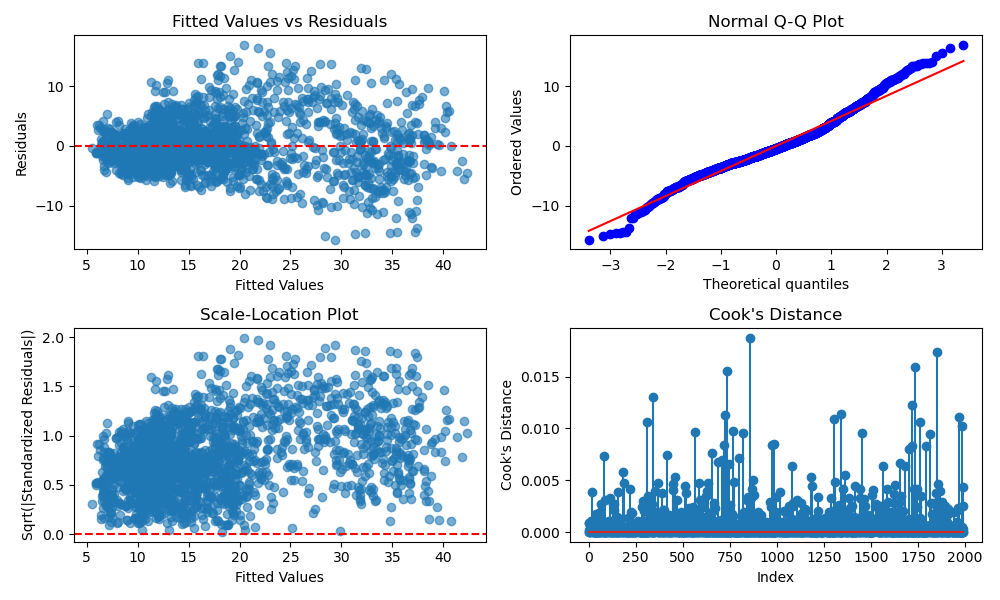
\includegraphics[width=1\textwidth]{Figure_7.png}
        \caption{检验误差}
        \label{fig:residual}
    \end{figure}
    \par
    \noindent \textbf{区间估计}
    \par
    使用 conf\_int( ) 函数可以得到回归系数的置信区间,如下所示:
    \begin{table}[H]
    \centering
    \begin{tabular}{|c|c|c|}
    \hline
    \textbf{变量} & \textbf{系数} & \textbf{95\% 置信区间} \\
    \hline
    常数项 (const) & -2.9848 & [-3.4719, -2.4978] \\
    \hline
    家庭社区病例指数平均值 (hh\_cmnty\_cli) & 0.8107 & [0.7928, 0.8286] \\
    \hline
    \end{tabular}
    \caption{回归系数的置信区间}
    \label{tab:conf_int}
    \end{table}
    \subsection{多元线性回归分析}
    同样地,我们可以通过调用 statsmodels 包中的 OLS 函数来进行多元线性回归分析。可以通过调用函数 summary( ) 来查看回归分析的结果。输出结果如下:
    \par
    \begin{tabular}{|l l l l|}
        \hline
        \textbf{依赖变量} & 测试阳性 (tested\_positive) & \textbf{R 平方} & 0.886 \\
        \textbf{模型} & OLS & \textbf{调整后的 R 平方} & 0.885 \\
        \textbf{方法} & 最小二乘法 (Least Squares) & \textbf{F 统计量} & 906.7 \\
        \textbf{日期} & 2024 年 12 月 25 日 & \textbf{F 统计量的 p 值} & 0.00 \\
        \textbf{时间} & 01:23:07 & \textbf{对数似然值} & -5136.8 \\
        \textbf{样本量} & 1994 & \textbf{Akaike 信息准则 (AIC)} & 10310 \\
        \textbf{残差自由度} & 1976 & \textbf{贝叶斯信息准则 (BIC)} & 10410 \\
        \textbf{模型自由度} & 17 & \textbf{协方差类型} & 非稳健 (nonrobust) \\
        \hline
        \end{tabular}
    \par   
    \begin{table}[H]
    \centering
    \begin{tabular}{|c|c|c|c|c|c|}
        \hline
        \textbf{变量} & \textbf{系数 (Coef.)} & \textbf{标准误差} & \textbf{t 值} & \textbf{p 值} & \textbf{95\% 置信区间} \\
        \hline
        const & 58.9312 & 3.875 & 15.210 & 0.000 & [51.333, 66.530] \\
        \hline
        cli & 5.1484 & 1.510 & 3.410 & 0.001 & [2.187, 8.110] \\
        \hline
        ili & -5.1648 & 1.480 & -3.490 & 0.000 & [-8.067, -2.263] \\
        \hline
        wnohh\_cmnty\_cli & -0.8288 & 0.108 & -7.663 & 0.000 & [-1.041, -0.617] \\
        \hline
        wbelief\_masking\_effective & -0.2443 & 0.050 & -4.918 & 0.000 & [-0.342, -0.147] \\
        \hline
        wbelief\_distancing\_effective & -0.3440 & 0.051 & -6.684 & 0.000 & [-0.445, -0.243] \\
        \hline
        wcovid\_vaccinated\_friends & 0.1536 & 0.021 & 7.220 & 0.000 & [0.112, 0.195] \\
        \hline
        wlarge\_event\_indoors & -0.1228 & 0.043 & -2.862 & 0.004 & [-0.207, -0.039] \\
        \hline
        wothers\_masked\_public & -0.2203 & 0.015 & -14.440 & 0.000 & [-0.250, -0.190] \\
        \hline
        wothers\_distanced\_public & 0.0529 & 0.044 & 1.203 & 0.229 & [-0.033, 0.139] \\
        \hline
        wshop\_indoors & -0.4513 & 0.040 & -11.385 & 0.000 & [-0.529, -0.374] \\
        \hline
        wrestaurant\_indoors & 0.0658 & 0.039 & 1.704 & 0.089 & [-0.010, 0.142] \\
        \hline
        wworried\_catch\_covid & -0.2097 & 0.032 & -6.479 & 0.000 & [-0.273, -0.146] \\
        \hline
        hh\_cmnty\_cli & 0.6886 & 0.140 & 4.933 & 0.000 & [0.415, 0.962] \\
        \hline
        nohh\_cmnty\_cli & 0.7545 & 0.169 & 4.458 & 0.000 & [0.423, 1.086] \\
        \hline
        wearing\_mask\_7d & 0.3688 & 0.022 & 16.890 & 0.000 & [0.326, 0.412] \\
        \hline
        public\_transit & -0.1314 & 0.048 & -2.724 & 0.006 & [-0.226, -0.037] \\
        \hline
        worried\_finances & -0.1086 & 0.025 & -4.340 & 0.000 & [-0.158, -0.060] \\
        \hline
    \end{tabular}
    \caption{多元线性回归分析结果}
    \label{tab:regression_results}
    \end{table}
    可见回归方程结果较好,大多数变量都通过了显著性检验,说明这些变量对测试阳性人数有显著影响。
    \par \noindent \textbf{变量选择}\par
    在代码中,我们实现了逐步回归算法,它是以 Akaike 信息准则(AIC)为准则的逐步回归算法,可以自动选择最优的变量组合。输出结果如下:                                           
最后删去了 wrestaurant\_indoors 变量,得到了最优的变量组合。结果如下\par 
\begin{tabular}{|l l l l|}
    \hline
    \textbf{依赖变量} & 测试阳性 (tested\_positive) & \textbf{R 平方} & 0.886 \\
    \textbf{模型} & OLS & \textbf{调整后的 R 平方} & 0.885 \\
    \textbf{方法} & 最小二乘法 (Least Squares) & \textbf{F 统计量} & 963.0 \\
    \textbf{日期} & 2024 年 12 月 25 日 & \textbf{F 统计量的 p 值} & 0.00 \\
    \textbf{时间} & 01:23:07 & \textbf{对数似然值} & -5137.5 \\
    \textbf{样本量} & 1994 & \textbf{Akaike 信息准则 (AIC)} & 10310 \\
    \textbf{残差自由度} & 1977 & \textbf{贝叶斯信息准则 (BIC)} & 10400 \\
    \textbf{模型自由度} & 16 & \textbf{协方差类型} & 非稳健 (nonrobust) \\
    \hline
\end{tabular}
此处相关回归分析放在附录,最后全部变量的 p 值均小于 0.05,说明这些变量对测试阳性人数有显著影响。
\par \noindent \textbf{回归诊断}\par
    首先画出残差和标准化残差的散点图,如下图所示:
    \begin{figure}[H]
        \centering
        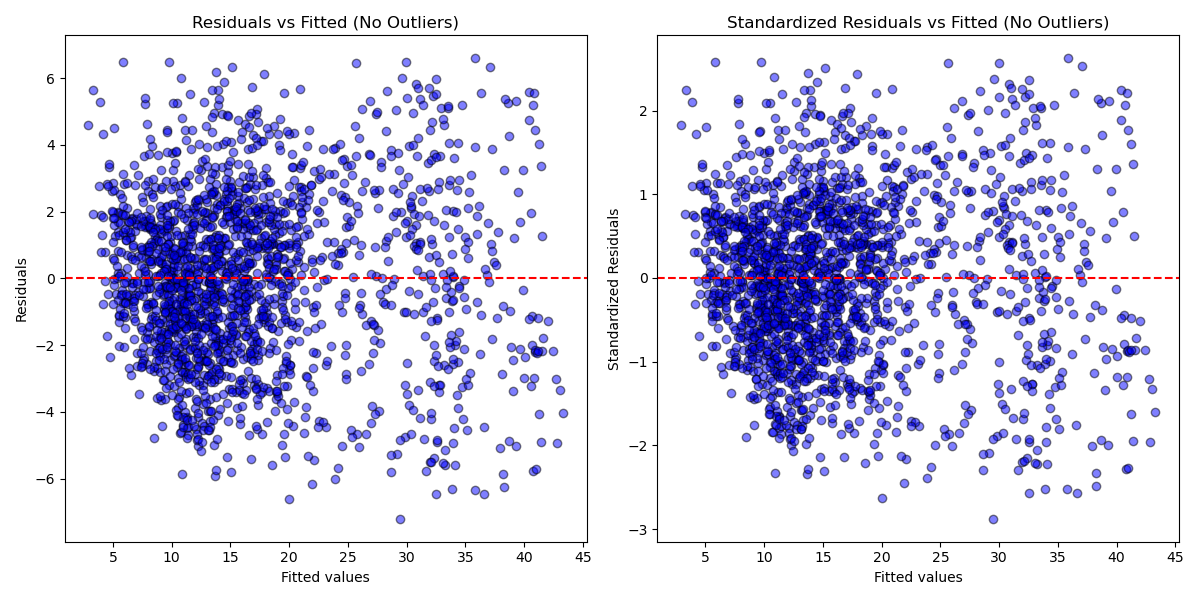
\includegraphics[width=1\textwidth]{Figure_8.png}
        \caption{残差和标准化残差的散点图}
        \label{fig:residuals}
    \end{figure}
    如果多元线性回归模型的假设成立,关于观测值的残差图中散点应该随机分布在 [-2,2] 之间里,
    此处大部分残差值在此范围内,说明模型的假设成立。
    \par
    \noindent \textbf{影响分析}\par
    从分析观测点对回归结果的影响入手,找出对回归结果影响很大的观测点
的分析方法称为影响分析。在 python 中,函数 get\_influence( ) 可以做回归诊断中影响分析的概括。输出结果见附录。
\newpage
\section{附录}
\subsection{修正后多元线性回归分析}
\begin{longtable}{|c|c|c|c|c|c|}
\hline
\textbf{变量} & \textbf{系数 (Coef.)} & \textbf{标准误差} & \textbf{t 值} & \textbf{p 值} & \textbf{95\% 置信区间} \\
\hline
\endfirsthead
\hline
\textbf{变量} & \textbf{系数 (Coef.)} & \textbf{标准误差} & \textbf{t 值} & \textbf{p 值} & \textbf{95\% 置信区间} \\
\hline
\endhead
\hline
const & 59.5500 & 3.841 & 15.505 & 0.000 & [52.018, 67.082] \\
\hline
cli & 5.3467 & 1.501 & 3.562 & 0.000 & [2.403, 8.291] \\
\hline
ili & -5.3542 & 1.472 & -3.639 & 0.000 & [-8.240, -2.468] \\
\hline
wnohh\_cmnty\_cli & -0.8331 & 0.108 & -7.705 & 0.000 & [-1.045, -0.621] \\
\hline
wbelief\_masking\_effective & -0.2454 & 0.050 & -4.941 & 0.000 & [-0.343, -0.148] \\
\hline
wbelief\_distancing\_effective & -0.3256 & 0.049 & -6.626 & 0.000 & [-0.422, -0.229] \\
\hline
wcovid\_vaccinated\_friends & 0.1455 & 0.020 & 7.209 & 0.000 & [0.106, 0.185] \\
\hline
wlarge\_event\_indoors & -0.1291 & 0.043 & -3.033 & 0.002 & [-0.213, -0.046] \\
\hline
wothers\_masked\_public & -0.2104 & 0.013 & -16.379 & 0.000 & [-0.236, -0.185] \\
\hline
wshop\_indoors & -0.4470 & 0.039 & -11.321 & 0.000 & [-0.524, -0.370] \\
\hline
wrestaurant\_indoors & 0.0557 & 0.038 & 1.477 & 0.140 & [-0.018, 0.130] \\
\hline
wworried\_catch\_covid & -0.2158 & 0.032 & -6.750 & 0.000 & [-0.279, -0.153] \\
\hline
hh\_cmnty\_cli & 0.6799 & 0.139 & 4.876 & 0.000 & [0.406, 0.953] \\
\hline
nohh\_cmnty\_cli & 0.7655 & 0.169 & 4.530 & 0.000 & [0.434, 1.097] \\
\hline
wearing\_mask\_7d & 0.3675 & 0.022 & 16.849 & 0.000 & [0.325, 0.410] \\
\hline
public\_transit & -0.1389 & 0.048 & -2.903 & 0.004 & [-0.233, -0.045] \\
\hline
worried\_finances & -0.1042 & 0.025 & -4.210 & 0.000 & [-0.153, -0.056] \\
\hline
\end{longtable}
\subsection{观测点}
Strong influence points based on Cook's Distance: [  13   41   43   51   53   58   65   84   89   99  112  134  136  154
  168  172  175  189  220  239  257  283  291  310  314  328  335  343
  355  410  452  457  469  499  516  520  552  566  586  589  594  595
  598  613  625  657  664  667  669  688  700  719  723  737  763  765
  767  773  777  799  819  820  821  837  858  866  872  954  965  967
  973  987  991 1038 1048 1055 1059 1062 1081 1086 1089 1096 1109 1131
 1133 1145 1149 1165 1172 1186 1217 1222 1236 1280 1288 1307 1311 1332
 1340 1352 1354 1365 1398 1407 1428 1445 1449 1454 1467 1496 1513 1532
 1543 1549 1551 1563 1583 1590 1591 1592 1597 1610 1622 1631 1654 1661
 1685 1716 1720 1734 1760 1764 1770 1796 1816 1818 1834 1845 1855 1860
 1862 1863 1951 1964 1970 1984]\par
High leverage points based on Leverage: [  51   65   89   92  141  151  164  175  210  239  240  247  261  305
  319  341  400  405  457  473  486  490  516  517  532  542  571  596
  606  634  771  791  799  822  866  873  889  980  990  991 1048 1062
 1086 1089 1138 1148 1172 1188 1236 1238 1244 1258 1302 1316 1326 1338
 1379 1397 1398 1463 1470 1483 1507 1513 1514 1517 1528 1529 1539 1568
 1603 1677 1740 1757 1760 1768 1788 1802 1819 1863 1870 1886 1986 1987]



    \end{document}